\documentclass[11pt,a4paper]{article}

\usepackage[utf8]{inputenc}
\usepackage[italian]{babel}
\usepackage{amsmath}
\usepackage{amsfonts}
\usepackage{geometry}
\geometry{a4paper, margin=2cm}
\usepackage{graphicx}

\title{
    \textbf{Elementi di Probabilità e Statistica per l'ICT \\
    Tesina Numero 1: Analisi di Rete con Wireshark
}}

\author{Andrea D'Amico \\ \small{Ingegneria Informatica (L-8) | Università degli studi di Catania}}
\date{}

\begin{document}

\maketitle

\tableofcontents

\section{Introduzione all'Analisi dei Pacchetti}
Sono stati catturati 200 pacchetti mediante il software Wireshark tramite l'interfaccia di rete \texttt{Ethernet}. I dati sono stati successivamente esportati in formato CSV per facilitare l'elaborazione tramite script Python. Questo elaborato descrive l'analisi statistica dei tempi di interarrivo e la distribuzione dei protocolli di rete.

Il dataset è composto da $N=200$ campioni prelevati dalla traccia \texttt{capture.pcapng}.

\section{Tempi di Interarrivo e Statistiche Descrittive}
Siano $t_1, t_2, \dots, t_{200}$ gli istanti temporali di arrivo dei pacchetti registrati. Definiamo tempo di interarrivo la variabile aleatoria:
\begin{equation}
    X(t_i) = t_i - t_{i-1} \quad \text{per } i = 2, \dots, 200.
\end{equation}

Il valore atteso (o media) della variabile aleatoria $X$ è definito tramite l'integrale:
\begin{equation}
    E[X] = \mu_X = \int_{-\infty}^{+\infty} x f_X(x) \, dx
\end{equation}
Inoltre, la varianza $\sigma_X^2$ può essere calcolata esplicitamente come la differenza tra il valore quadratico medio $m_X^2 = E[X^2]$ e la media teorica al quadrato:
\begin{align}
    \sigma_X^2 & = m_X^2 - \mu_X^2
    = \left( \int_{-\infty}^{+\infty} x^2 f_X(x) \, dx \right) - \mu_X^2
\end{align}

Dato che la traccia acquisita è formata da dati discreti e finiti, per il calcolo delle deviazioni e delle statistiche campionarie sui $199$ intertempi si è sfruttata la libreria standard di Python:
\begin{verbatim}
import statistics
inter_arrival_times = [times[i] - times[i-1] for i in range(1, len(times))]

mean_iat = statistics.mean(inter_arrival_times)
stdev_iat = statistics.stdev(inter_arrival_times)
\end{verbatim}

I risultati ottenuti dall'elaborazione numerica sono riassunti nella seguente tabella:

\begin{table}[h]
    \centering
    \begin{tabular}{lr}
        \hline\hline
        \textbf{Parametro Statistico}         & \textbf{Valore [secondi]} \\
        \hline
        Media Campionaria ($\bar{x}$)         & 0.067018                  \\
        Mediana ($Q_2$)                       & 0.009945                  \\
        Deviazione Standard Campionaria ($s$) & 0.155533                  \\
        \hline\hline
    \end{tabular}
    \caption{Indici di posizione e variabilità dei tempi di interarrivo.}
\end{table}

C'è una differenza sostanziale tra media e mediana. Questo succede spesso nel traffico di rete reale, per via dei pacchetti "burst" che arrivano vicinissimi tra di loro, seguiti da pause lunghe che alterano la distribuzione.

\subsection{Frequenze Cumulative}
Per un modello continuo la Funzione di Distribuzione Cumulativa (CDF) può essere riscritta come:
\[ F_X(x) = P(X \leq x) = \int_{-\infty}^{x} f_X(t) \, dt \]

Attraverso il calcolo numerico in Python e l'uso di librerie grafiche, è stata tracciata la CDF empirica al fine di mostrare l'andamento della probabilità cumulativa dei dati:
\begin{verbatim}
sorted_iat = np.sort(inter_arrival_times)
y_values = np.arange(len(sorted_iat)) / float(len(sorted_iat) - 1)
plt.plot(sorted_iat, y_values, marker='.', linestyle='none')
\end{verbatim}

Il grafico risultante è il seguente:

\begin{figure}[h]
    \centering
    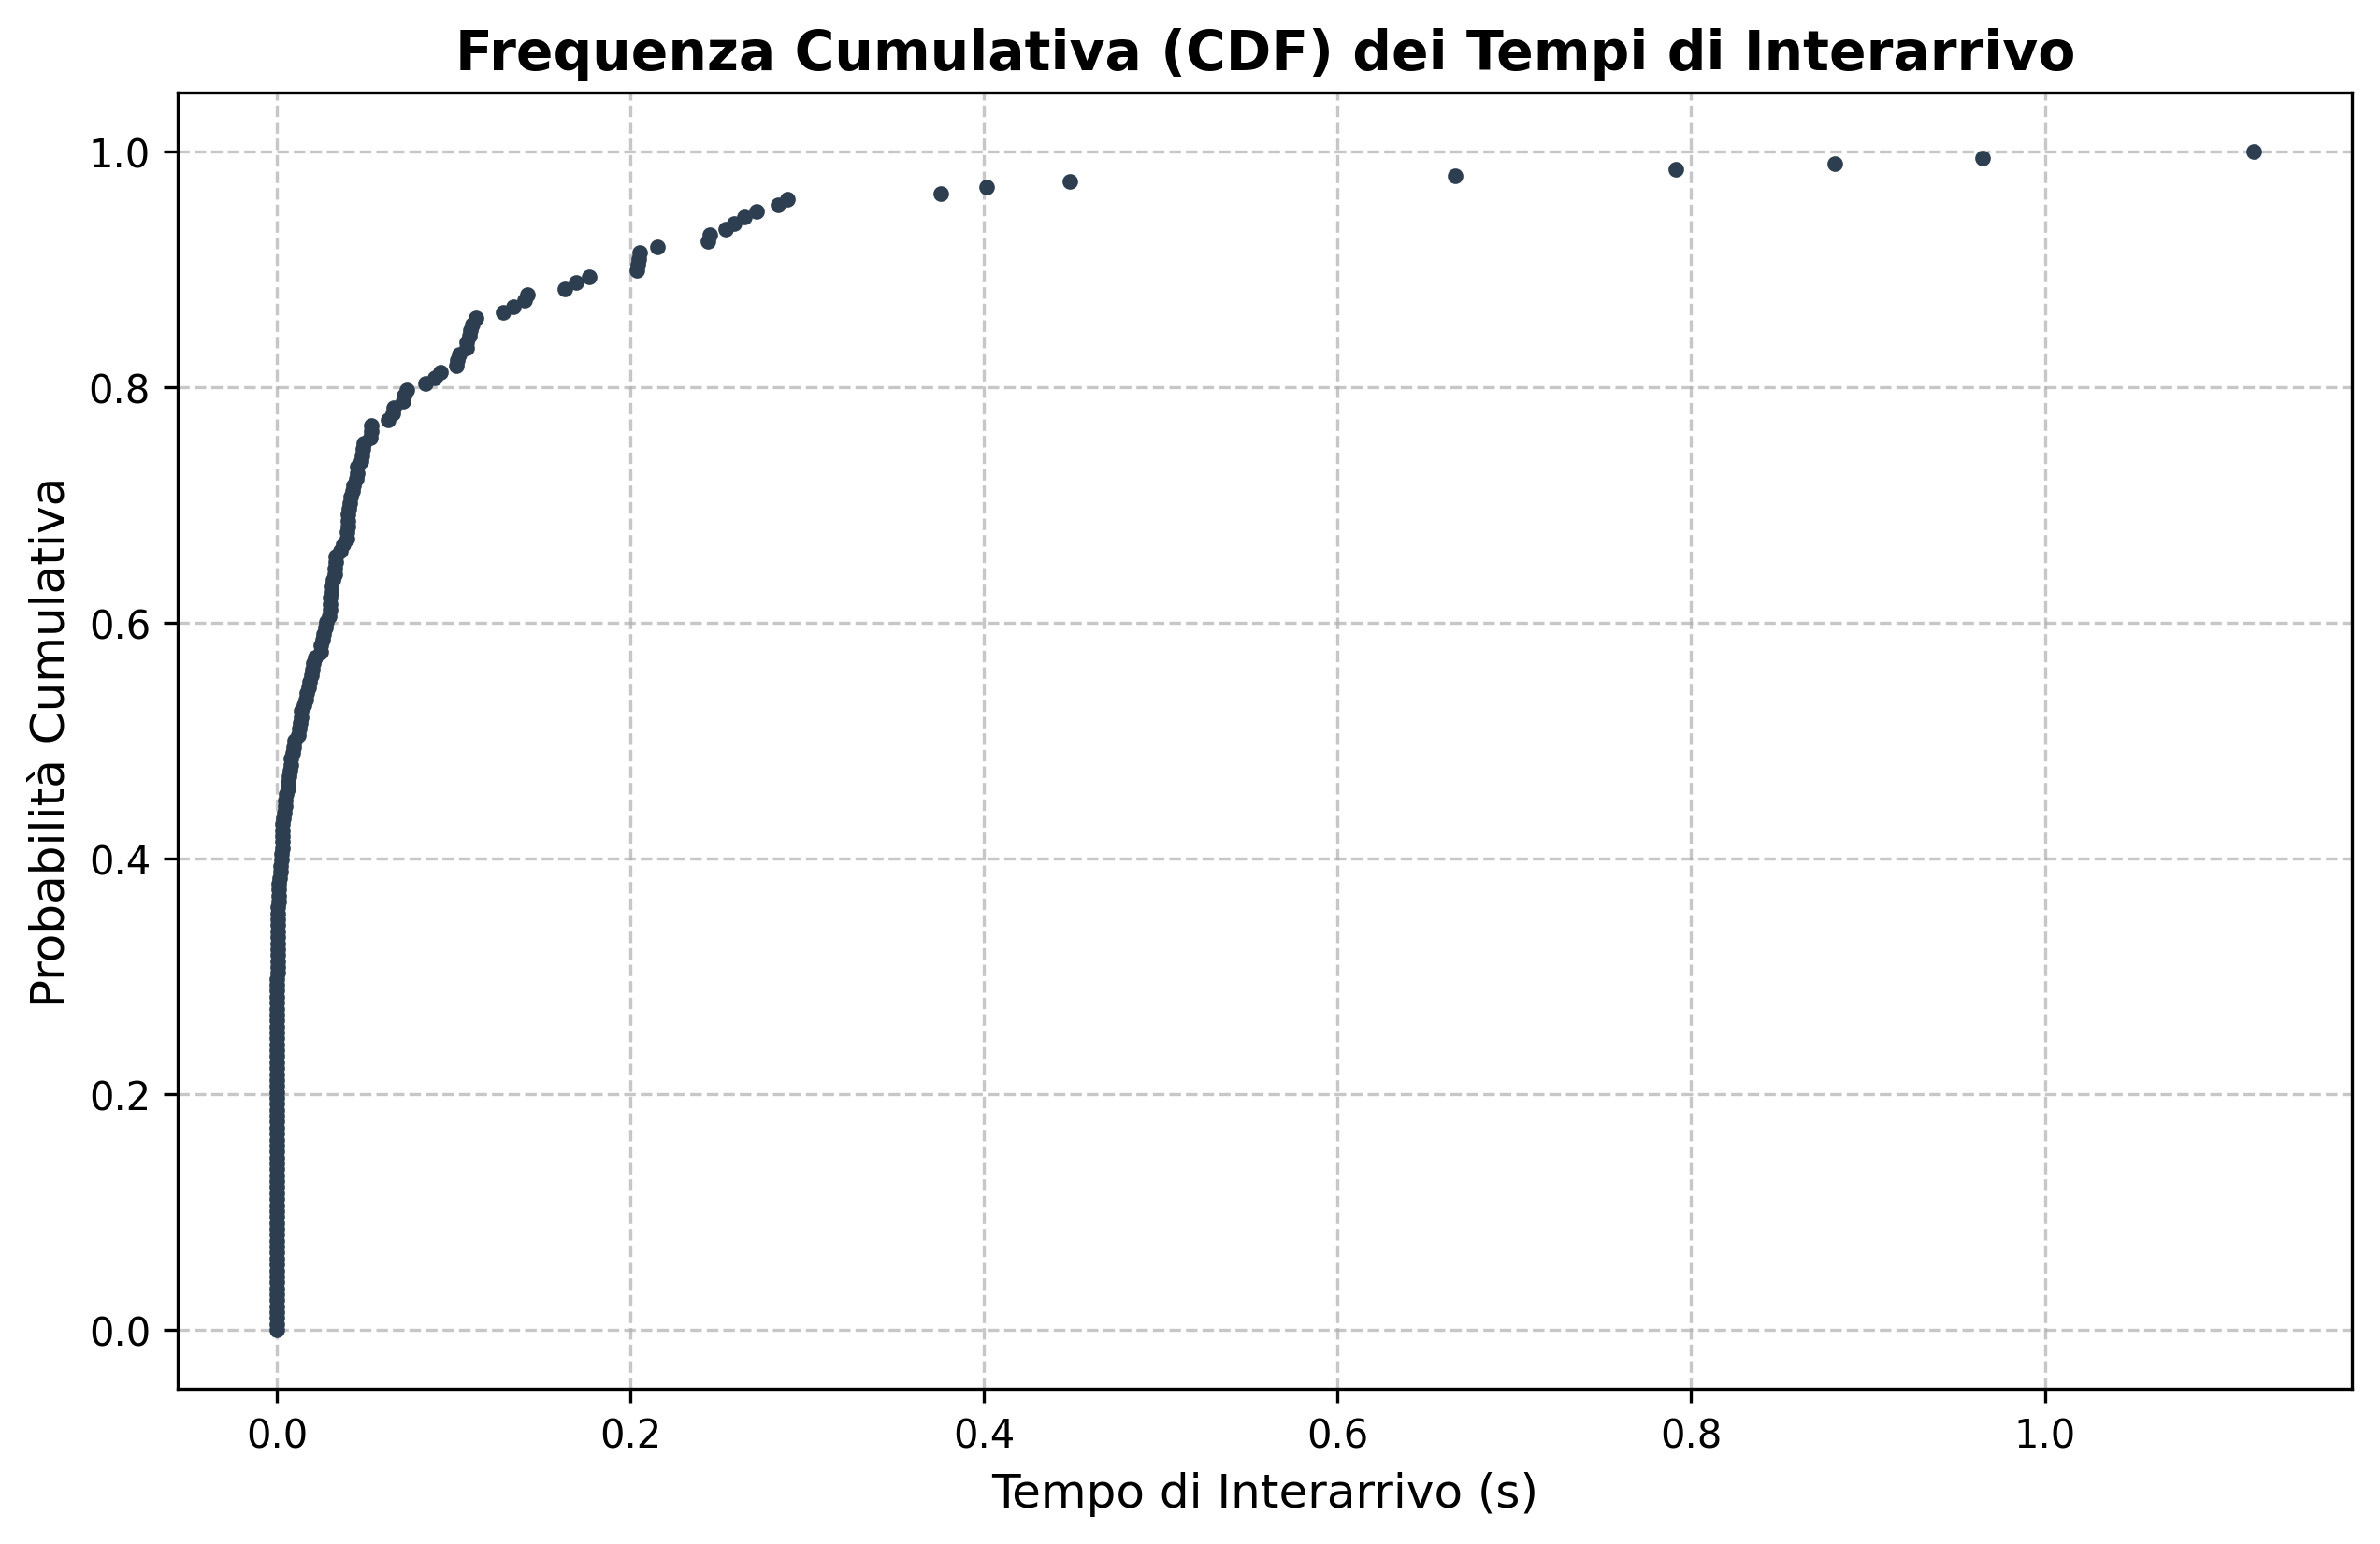
\includegraphics[width=0.55\textwidth]{cdf_interarrival.png}
    \caption{Grado di probabilità cumulativa per i tempi di interarrivo dei pacchetti catturati.}
\end{figure}

\newpage
\section{Classificazione per Tipo di Protocollo}
L'analisi successiva è mirata ad identificare le tipologie di protocolli presenti nella sessione catturata. Ad esempio il DNS e l'ARP, protocolli fondamentali, risultano rilevati in quantità significative nel traffico ordinario.

La tabella seguente riporta il conteggio dei principali protocolli estratti dal file CSV:

\begin{center}
    \begin{tabular}{lc}
        \hline\hline
        \textbf{Protocollo} & \textbf{Conteggio Pacchetti} \\
        \hline
        TCP                 & 60                           \\
        UDP                 & 28                           \\
        TLSv1.2             & 28                           \\
        DNS                 & 24                           \\
        ARP                 & 22                           \\
        Altri               & 38                           \\
        \hline\hline
    \end{tabular}
\end{center}

\subsection{Istogramma dei Protocolli}
L'istogramma evidenzia in modo chiaro come il traffico complessivo sia fortemente dominato dal TCP, protocollo di livello trasporto impiegato tipicamente per garantire l'assenza di perdite.

\begin{figure}[h]
    \centering
    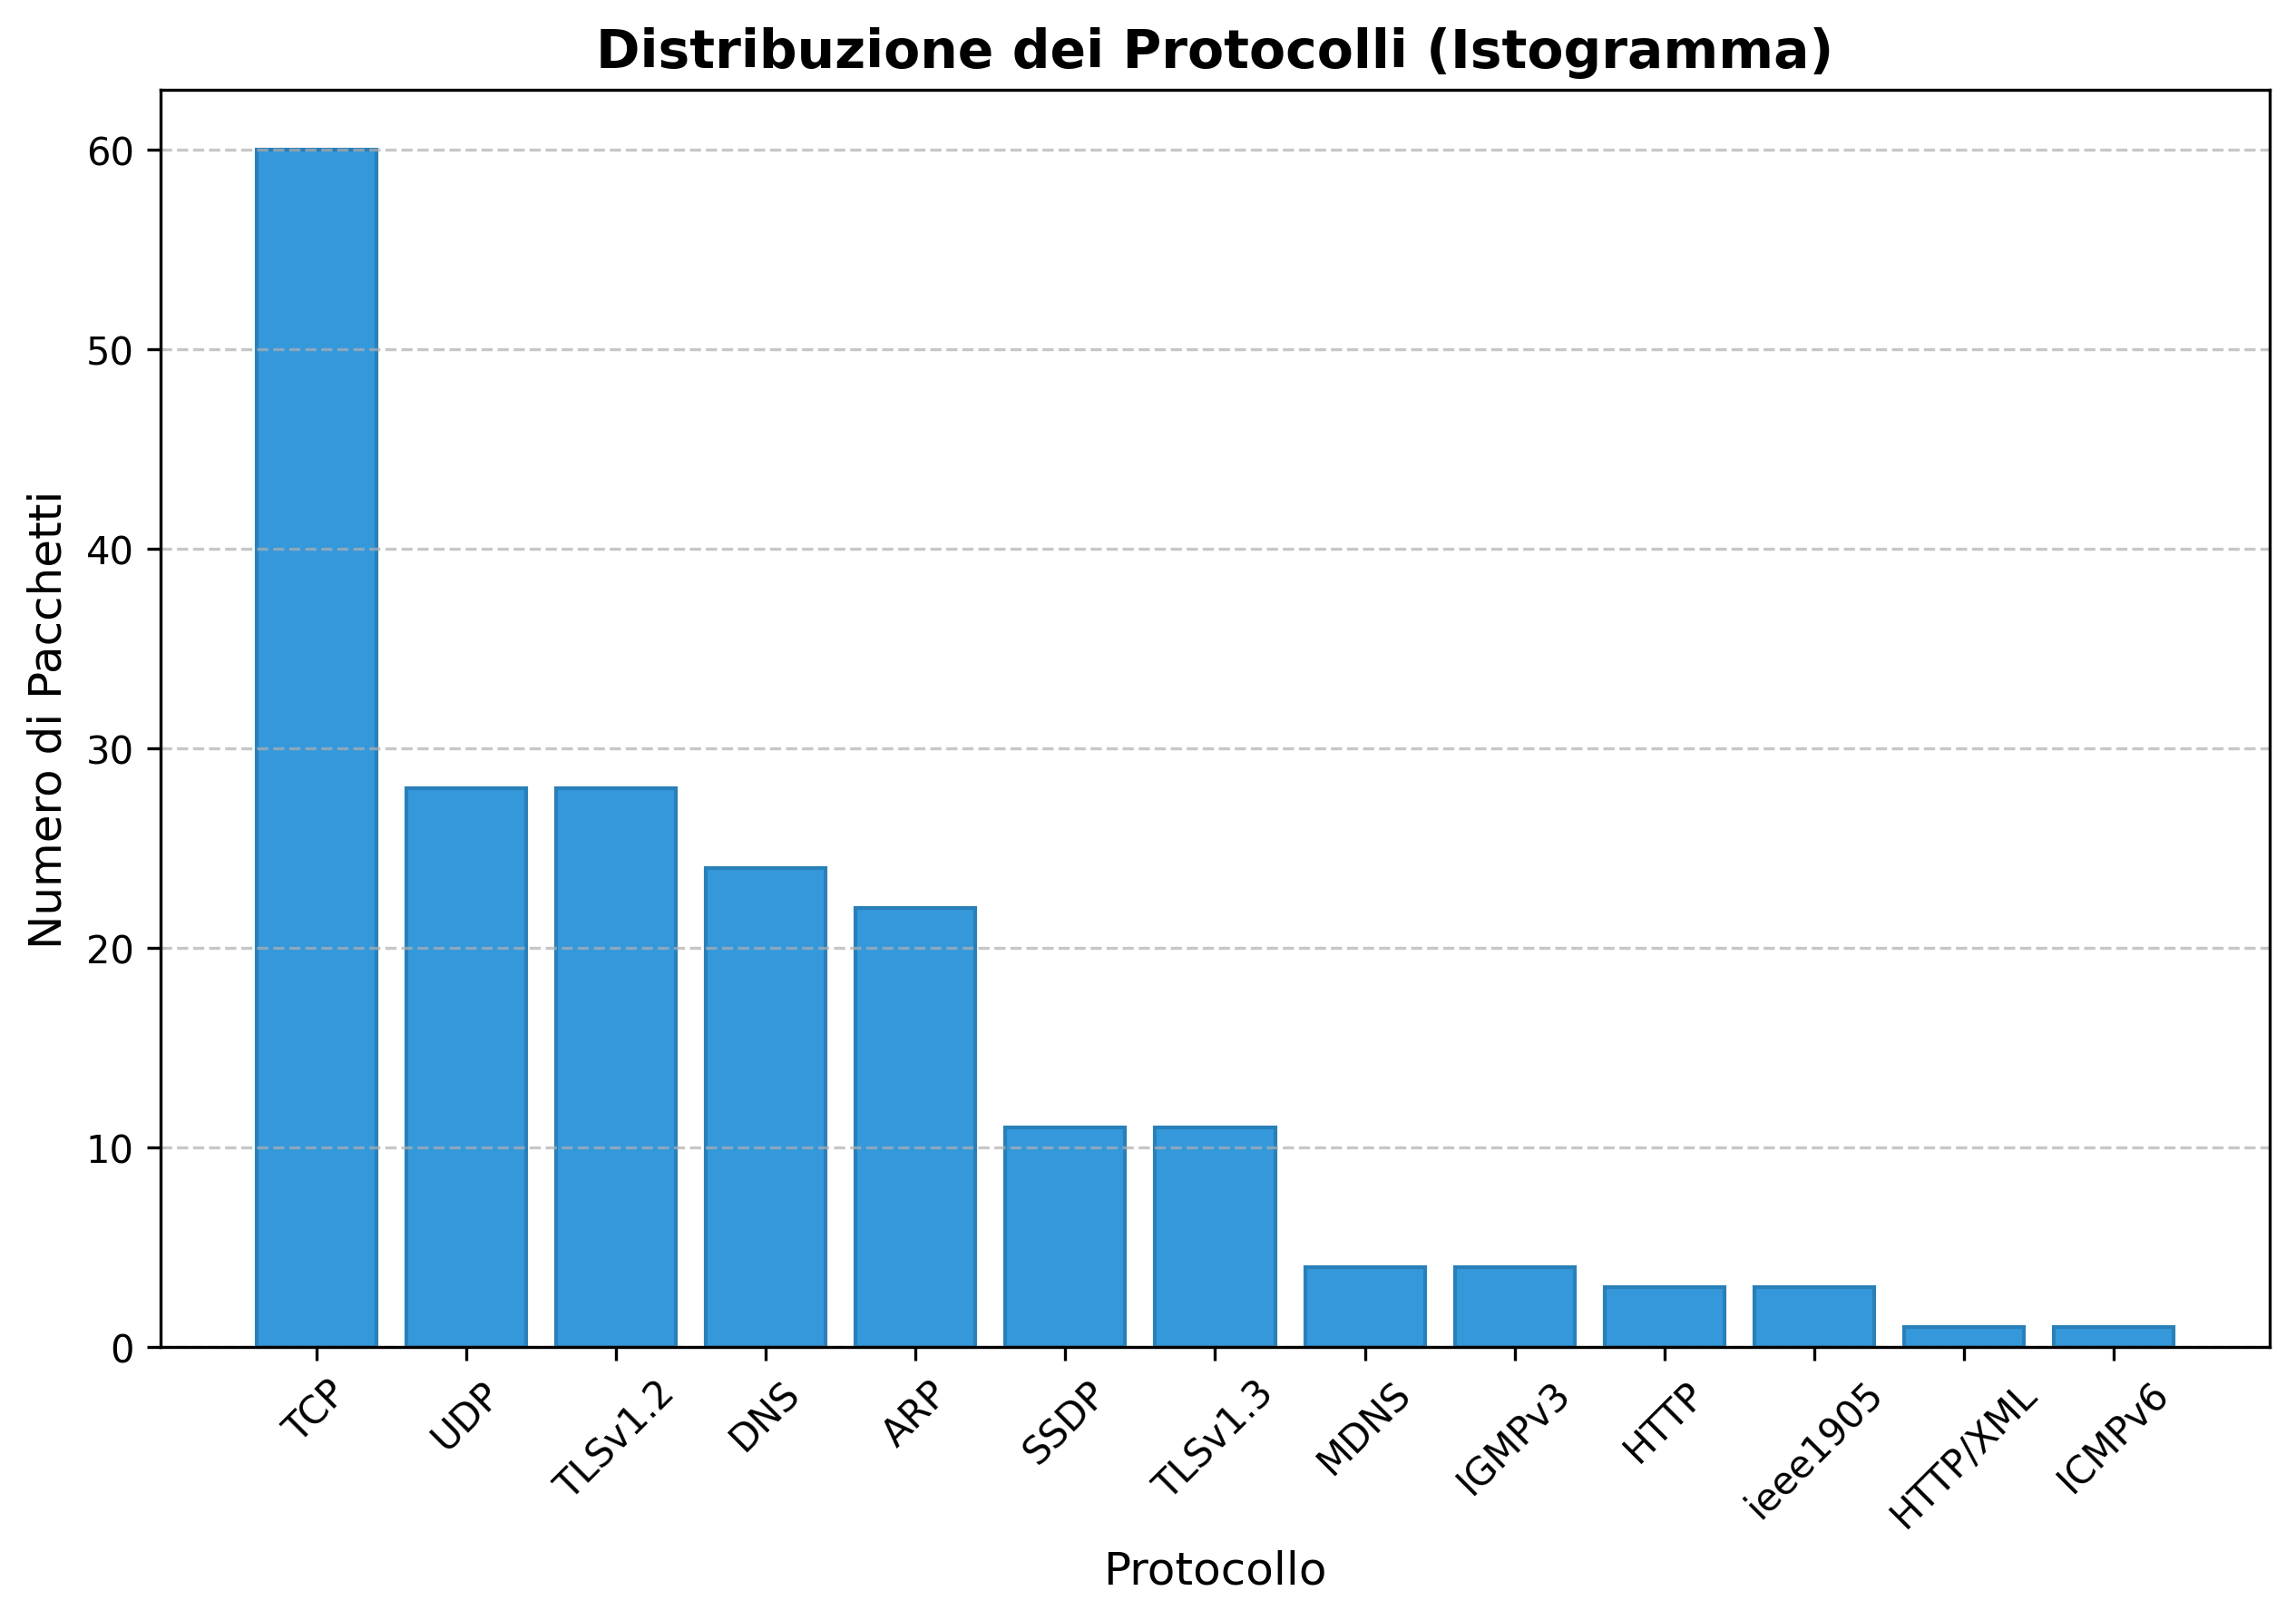
\includegraphics[width=0.60\textwidth]{protocol_histogram.png}
    \caption{Distribuzione del numero di pacchetti per tipologia di protocollo.}
\end{figure}

\subsection{Distribuzione Percentuale}
La suddivisione percentuale è rappresentata tramite un grafico a torta. In fase di generazione grafica dello script, è stata applicata una logica condizionale al fine di aggregare i protocolli minoritari sotto la dicitura unica "Others", migliorandone dunque la leggibilità:
\begin{verbatim}
if len(sorted_protos) > 6:
    top_protos = list(sorted_protos.items())[:5]
    others_count = sum(count for label, count in list(sorted_protos.items())[5:])
\end{verbatim}

\begin{figure}[h]
    \centering
    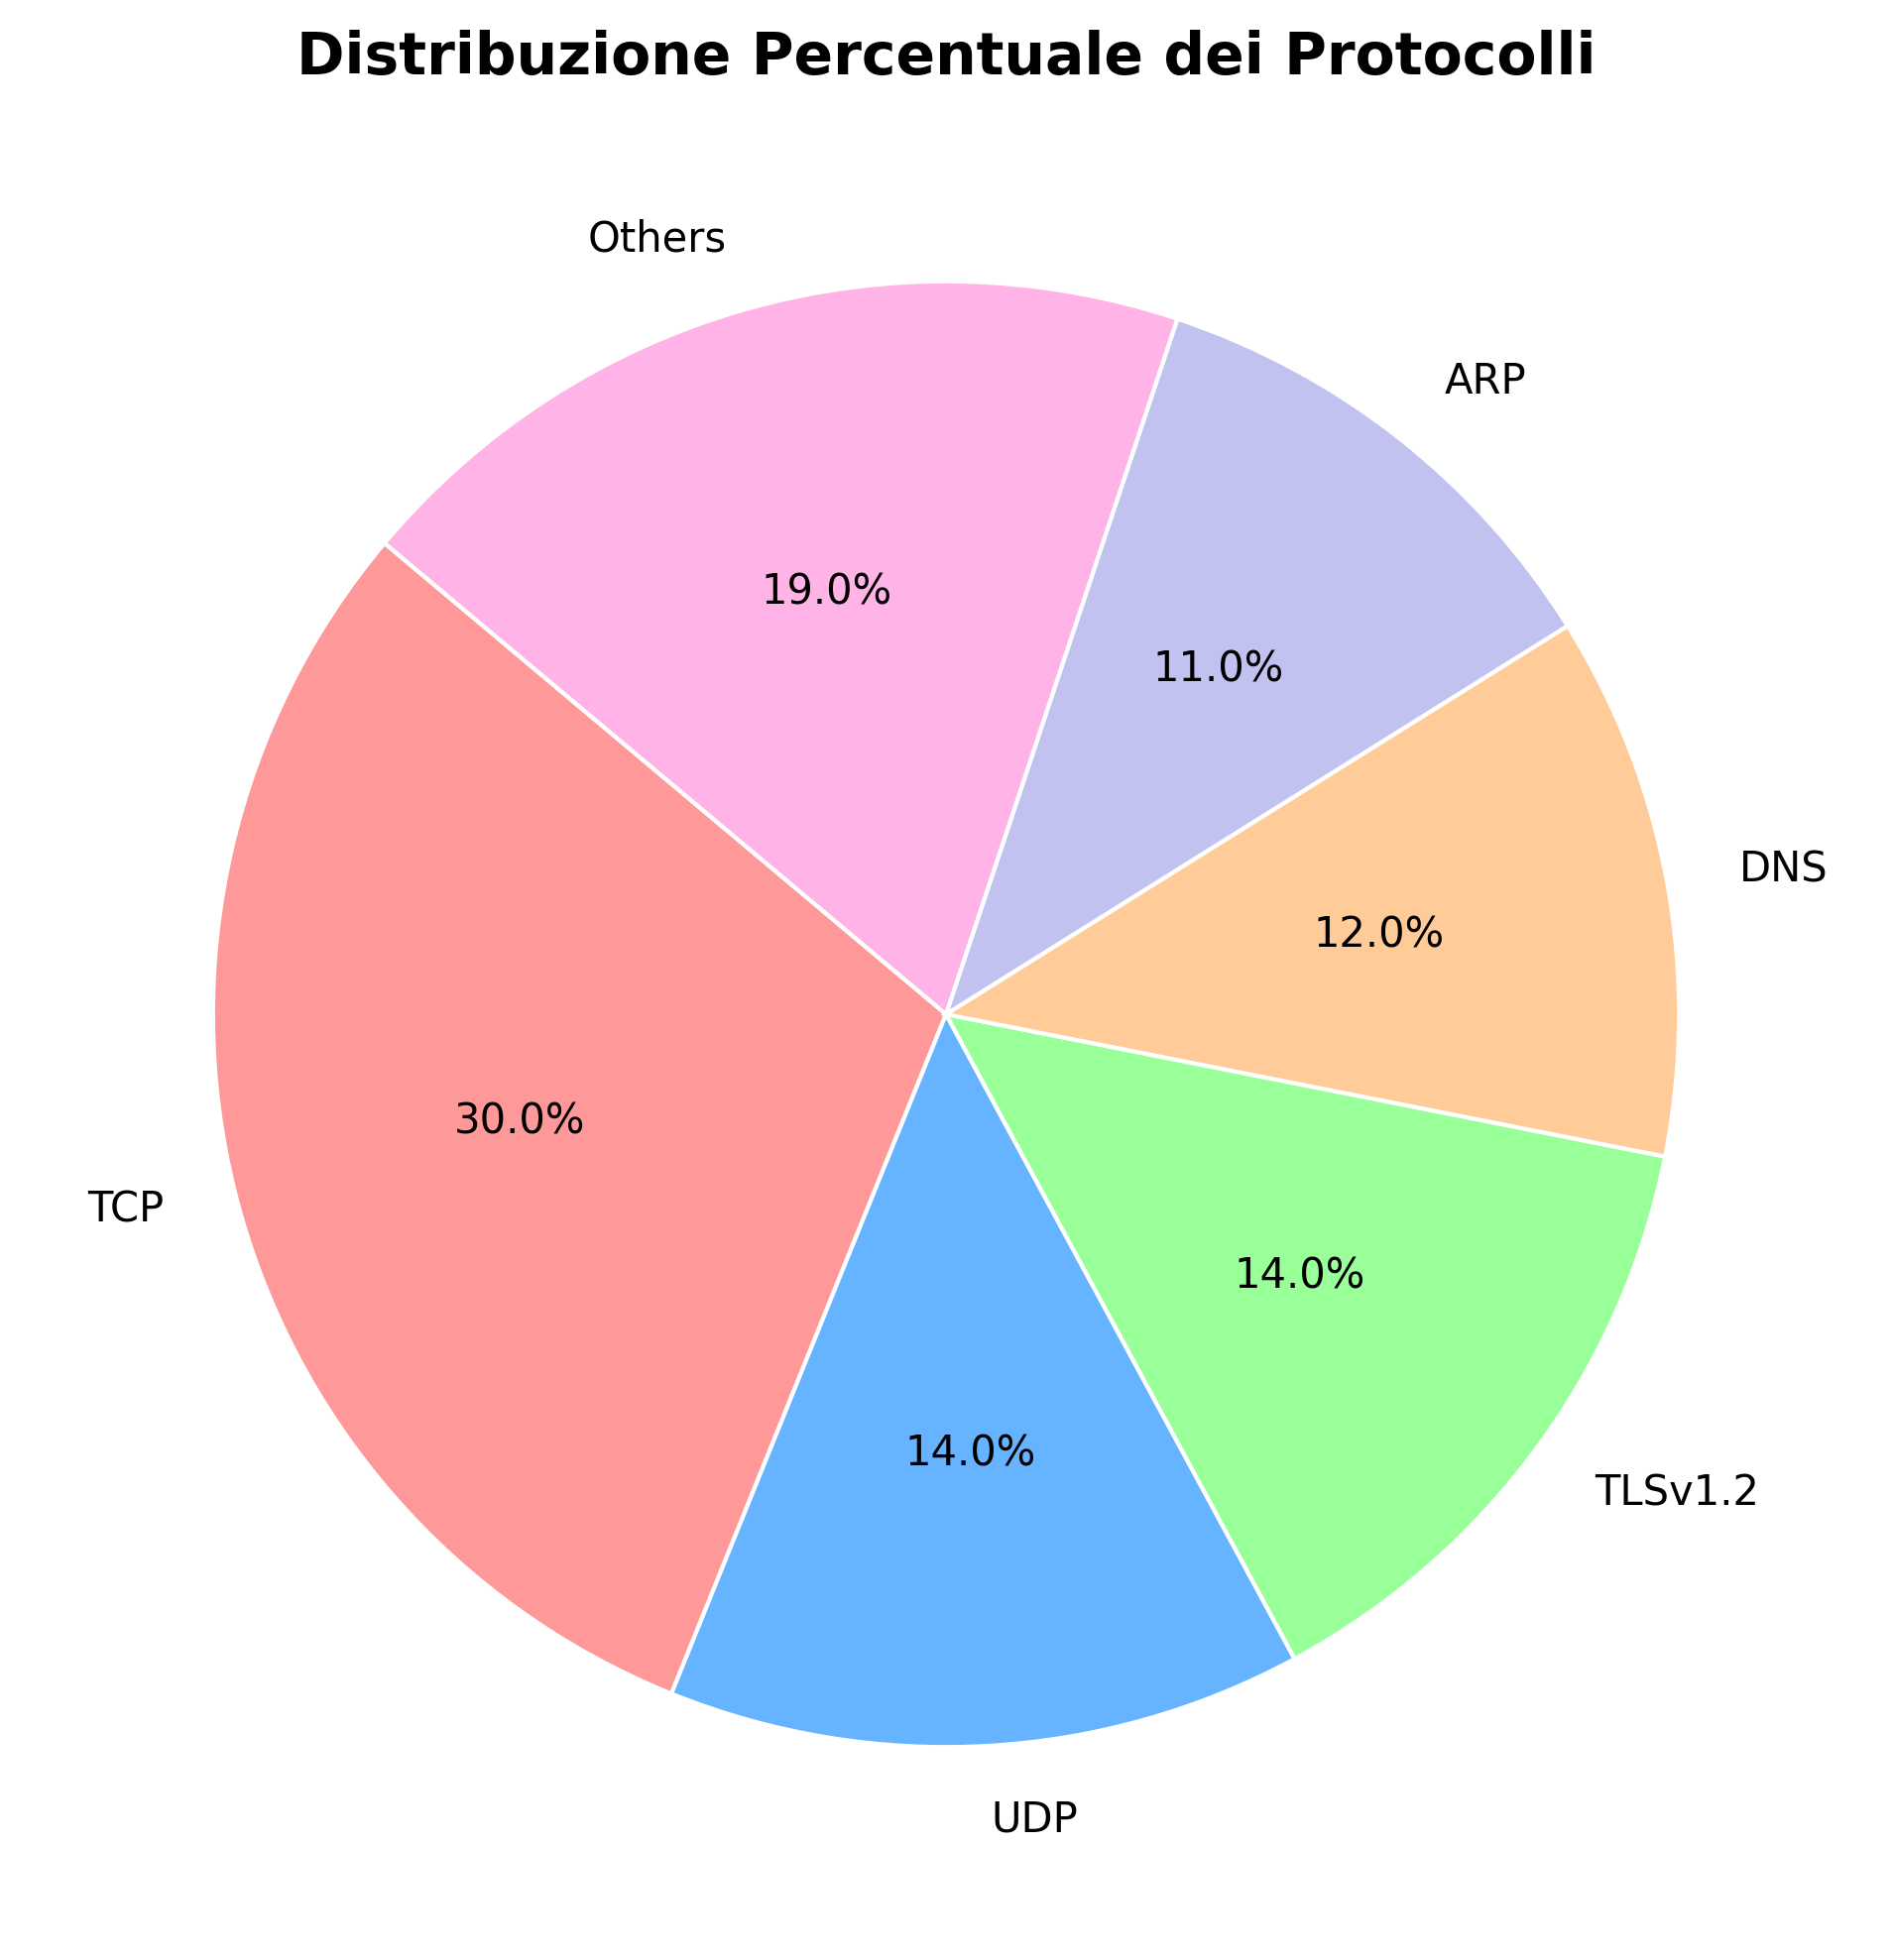
\includegraphics[width=0.45\textwidth]{protocol_pie.png}
    \caption{Ripartizione percentuale dei protocolli catturati.}
\end{figure}

\section{Conclusioni}
In conclusione, i dati raccolti indicano un flusso temporale per nulla omogeneo, presentando una variabilità elevata rispetto ai valori medi ($s = 0.155$ s a fronte di una media $\bar{x} = 0.067$ s). Queste evidenti fluttuazioni sono coerenti con una sessione di normale navigazione web. Infine, la netta predominanza del traffico TCP conferma pienamente questa destinazione d'uso.

\vfill
\begin{center}
    \rule{0.6\textwidth}{0.4pt} \\
    \vspace{0.2cm}
    \small{\textit{Questo documento e il relativo codice sono ospitati all'interno di un repository pubblico su GitHub.}} \\
    \vspace{0.1cm}
    \textbf{\texttt{https://github.com/andreadamico678/tesine-teoria-dei-segnali}}
\end{center}


\end{document}
